
%(BEGIN_QUESTION)
% Copyright 2011, Tony R. Kuphaldt, released under the Creative Commons Attribution License (v 1.0)
% This means you may do almost anything with this work of mine, so long as you give me proper credit

This combustion burner air/fuel ratio control strategy does not work very well.  It fails to hold the actual ratio of air flow to fuel flow at the desired proportion throughout the firing command signal range:

$$\includegraphics[width=15.5cm]{i03846x01.eps}$$

Re-draw a practical ratio control system that will maintain a stable air/fuel flow ratio under all conditions.  Note: you do not have to go to the extent of providing cross-limiting of air and fuel flows -- a simple ratio system will suffice:

$$\includegraphics[width=15.5cm]{i03846x02.eps}$$

\underbar{file i03846}
%(END_QUESTION)





%(BEGIN_ANSWER)

Here is one solution:

$$\includegraphics[width=15.5cm]{i03846x03.eps}$$

{\it Half credit if the ratio setpoint for the captive flow controller comes off the wild flow's valve position rather than its flow transmitter signal.}

%(END_ANSWER)





%(BEGIN_NOTES)


%(END_NOTES)


